% DOCUMENTO
% !TEX root = relative/or/absolute/path/to/root/main.tex
% !BIB program = biblatex
\documentclass[12pt]{article}
% Language setting
% Replace `english' with e.g. `spanish' to change the document language
\usepackage[spanish,es-tabla]{babel}
\usepackage[utf8]{inputenc}
\usepackage[T1]{fontenc}
% font
\usepackage{lmodern}
\usepackage[T1]{fontenc}
\usepackage{heuristica}
\usepackage[heuristica,vvarbb,bigdelims]{newtxmath}
\renewcommand*\oldstylenums[1]{\textosf{#1}}
\let\Bbbk\relax
% Set page size and margins
% Replace `letterpaper' with`a4paper' for UK/EU standard size
\usepackage[a4paper,margin=1.7cm]{geometry}
\usepackage{setspace}
\onehalfspacing
\setlength{\parskip}{2mm plus 0.5mm minus 1mm}

% MATEMÁTICA
\usepackage{amssymb,amsmath}
\usepackage{booktabs}
\usepackage[es-tabla]{babel}

% REFERENCIAS
\usepackage[colorlinks=true, allcolors=blue]{hyperref}
\usepackage[spanish,nameinlink]{cleveref}
\crefname{table}{Tabla}{Tablas}
\crefname{section}{sección}{secciones}
\crefname{subsection}{subsección}{subsecciones}
\crefname{equation}{ec.}{ecs.}

% BIBLIOGRAFÍA
\usepackage{biblatex} %Imports biblatex package
\addbibresource{sample.bib} %Import the bibliography file
\usepackage{csquotes}

% FIGURAS
\usepackage{graphicx}
\usepackage{float}
\usepackage{subfig}
\floatplacement{figure}{h}
\usepackage{chngcntr}
% \counterwithin{figure}{section}
\usepackage{placeins}
\usepackage[justification=centering,labelfont=bf]{caption}


\title{Estimación de la incertidumbre de medición}
\author{Paula Martínez Garbino}

\begin{document}
\maketitle
% \begin{abstract}
% Your abstract.
% \end{abstract}
\section{Introducción}

El resultado de una calibración sólo se encuentra completo cuando el valor medido es acompañado de su incertidumbre de medición junto a una declaración del factor de cobertura, intervalo de confianza y distribución de probabilidad. En este documento se resumen informalmente tanto el proceso general de evaluación de incertidumbre como el método empleado para distintas magnitudes bajo el alcance de AKRIMET, enunciando con sus referencias los modelos matemáticos y conceptos de estadística necesarios en cada caso.\cite{GUM}

\section{Metodología general para la evaluación de incertidumbres}

\subsection{Modelo matemático del mensurando}

En la mayor parte de los casos, un mensurando o _magnitud de salida_ $Y$ que se busca reportar como resultado de una medición o calibración no se mide directamente, sino que se determina a partir de otras $N$ _magnitudes de entrada_ $X_1, X_2, \ldots, X_N$, por medio de una relación funcional $f$:
\begin{equation}
    Y = f(X_1, \ldots, X_N).    
\end{equation}

**[GUM 4.1.1, p.11 ec. (1)]**

Las magnitudes de entrada de las que depende la magnitud de salida pueden ser consideradas a su vez como mensurandos dependientes de otras magnitudes, junto con las _correcciones_ y _factores de corrección_ por efectos sistemáticos. **[GUM 4.1.2, 4.1.3]** $f$, entonces, es la función que contiene toda magnitud, incluyendo correcciones y factores de corrección, susceptible de contribuir a una componente significativa de la incertidumbre del resultado de medida. Para la determinación de $f$ se identifican todas estas variables de influencia, incluyendo aquellas que son despreciables en corrección pero sí son considerables en su incertidumbre y se toma una decisión informada sobre cuáles son significativas o despreciables a partir del modelo físico conocido del mensurando $Y$ y de métodos experimentales.

La combinación de la relación funcional $f$ y el conjunto de las magnitudes de entrada, las correcciones y las _componentes de incertidumbre_ que contribuyen a la incertidumbre del resultado de medición determinan el _modelo matemático_ de la calibración.

### 1.2. Evaluación del resultado de medición y componentes de incertidumbre

La evaluación (asignación de valores) o estimación de las magnitudes de entrada y componentes de incertidumbre puede determinarse a partir mediciones y métodos estadísticos o importarse de fuentes externas e información disponible previamente (libros, papers, certificados, etc.). **[GUM 4.1.3]**

El resultado de la medición $y$ es una _estimación_ del mensurando $Y$, que se obtiene introduciendo las $N$ estimaciones de entrada $x_1, x_2, \ldots, x_N$ para los valores de las $N$ magnitudes $X_1, X_2, \ldots, X_N$ en la ecuación **[]**:

$$
y = f(x_1, \ldots, x_N).
$$
**[GUM 4.1.4, p.12 ec. (2)]**

La desviación estándar estimada asociada a $y$, denominada _incertidumbre estándar combinada_ o _incertidumbre combinada_ y representada por $u_c(y)$, se determina a partir de la desviación estándar estimada asociada a cada estimación de entrada $x_i$, denominada _incertidumbre estándar_ y representada por $u(x_i)$ o $\sigma(x_i)$. **[GUM 4.1.5, p.12]**. Cada $x_i$ y su $\sigma(x_i)$ provienen de una distribución de valores posibles (distribución de probabilidad) observada o supuesta en base a la información conocida de la magnitud de entrada $X_i$. **[GUM 4.1.6, p.12]** y tienen un número de grados de libertad asociado.

#### 1.2.1. Factor de estandarización

La forma y el ancho de la distribución de probabilidad de origen determinan el _factor de estandarización_ por el cual debe dividirse el valor numérico de cada componente de incertidumbre para obtener la incertidumbre estándar correspondiente.

$$
\sigma(x_i) = \frac{\Delta_{\textit{componente}}}{\textit{factor}},
$$

donde llamo $\Delta$ al valor numérico de la componente de incertidumbre sin estandarizar.



| Distribución | Valor dado como | Factor | Fuente |
|---|---|---|---|
| Normal | desviación típica | 1 | `GUM 4.3.3, p.15` |
| Rectangular | ancho completo de la campana `2a` | `2√3` | `GUM 4.3.7-4.3.8, p.15-16` |
| Rectangular | medio ancho de la campana `a` | `√3` | `GUM 4.3.7, p.16` ec. (7) |
| Triangular | ancho completo de la campana `2a` | `2√6` | `GUM 4.3.9, p.17` ec. (9b) |
| Triangular | medio ancho de la campana`a` | `√6` | `GUM 4.3.9, p.17` ec. (9b) |

#### 1.2.2. Tipos de incertidumbre y grados de libertad

Las componentes de incertidumbre se clasifican por su método de evaluación en incertidumbres de tipo A y de tipo B.

Las incertidumbres de tipo A son aquellas que se obtienen mediante el análisis estadístico de serie de observaciones. **[GUM 4.2]** El número de grados de libertad para incertidumbres de este tipo es $\nu = n - m$, donde n es el número de observaciones y m el número de restricciones involucradas en la estimación. **[GUM 4.2, G.3.3]**

Las incertidumbres de tipo B son aquellas que se obtienen por cualquier otro método que no sea el análisis estadístico de observaciones **[GUM 4.3]**. Para las incertidumbres de tipo B el grado de libertad es infinito **[GUM G.6.4]**, aunque en la práctica basta con asumir $\nu \approx 100$.

### 1.3. Determinación de la incertidumbre combinada

La incertidumbre combinada se calcula componiendo las incertidumbres estándar de las estimaciones $x_i$ a través de la _ley de propagación de incertidumbres_

$$
u_c(y) = \sqrt{\sum^{N}_{i=1} \left(\dfrac{\partial f}{\partial x_i}\right)^2 \sigma^2(x_i)} = \sqrt{\sum^{N}_{i=1} c_i^2 \sigma^2(x_i)} ,
$$

donde $ci = \left. \left( \dfrac{\partial f}{\partial X_i}\right ) \right|_{x_i} \equiv \dfrac{\partial f}{\partial x_i}$ es el _coeficiente de sensibilidad_ de la componente, un parámetro que describe cuán sensible es el resultado de la medición a variaciones en la magnitud de entrada $x_i$. Los $c_i$ también pueden calcularse de forma experimental.
[**GUM 5.1.1, 5.1.2, 5.1.3**]

### 1.4. Determinación de la incertidumbre expandida

Para satisfacer las necesidades de determinadas aplicaciones industriales y comerciales, la incertidumbre combinada $u_c(y)$ se multiplica por un factor de cobertura $k$, obteniéndose la denominada _incertidumbre expandida_

$$
U = k . u_c(y).
$$

U define un intervalo $y - U$ a $y + U$ alrededor del resultado de medición que comprende una fracción $p$ de la distribución de probabilidad de salida de $y$ y $u_c(y)$. $p$ es el _nivel de confianza_ o _probabilidad_ del intervalo, la probabilidad de que el valor "verdadero" de la magnitud de salida $Y$ se encuentre dentro de ese intervalo (probabilidad de que $y-U\leq Y \leq y+U$). 
**[GUM 6.2]**

#### 1.4.1. Elección de $k$ y distribución t-Student

El factor de cobertura requerido para asegurar un nivel de confianza $p$ en el intervalo $y - U$ a $y + U$ depende de la distribución de probabilidad de la magnitud de salida **[GUM 6.3.2]**, por ejemplo, para la distribución normal $k=2$ corresponde a un nivel aproximado de confianza 95%. En general esta distribución no se conoce porque resulta de la convolución de las distribuciones de probabilidad de todas las magnitudes de entrada, lo que requiere un amplio conocimiento de cada una de ellas y cálculos extensos de combinación de distribuciones. Se acepta su aproximación por la distribución t-Student de $\nu_{eff}$ grados de libertad, donde $\nu_{eff}$ son los grados de libertad efectivos de $u_c(y)$ **[GUM G.6.2]**, calculados con la fórmula de Welch-Satterthwaite

$$
\nu_{eff} = \frac{u_c^4(y)}{\sum^N_{i=1}[\frac{u_i^4(y)}{\nu_i}]},
$$

con $u_i(y) = |c_i|u(x_i)$. **[GUM G.4.1]** El factor $k$ se obtiene como $t_p(\nu_{eff})$ el valor crítico para un nivel de confianza $p$ a dos colas obtenido directamente de la función de probabilidad acumulada inversa de la distribución t-Student de $\nu_{eff}$ grados de libertad. De esta forma
$$
U = k_p.u_c(y) = t_p(\nu_{eff}).u_c(y).
$$

La distribución de Welch-Satterthwaite tiende a la distribución normal cuando $\nu \longrightarrow \inf$. Para un nivel de confianza $p = 95\%$, si se obtiene $k_p<2$ se considera que la distribución de salida está bien aproximada por la distribución normal, de modo que en ese caso se elige en su lugar $k=2$ para reportar la incertidumbre expandida con un nivel aproximado de confianza del 95% bajo la distribución normal. 
**[GUM G.6.6]**

### 1.5. Otros resultados

Ya sea para validar los cálculos de estimación de la incertidumbre o para reportarlo en el certificado de calibración, hay otros resultados aparte de la incertidumbre expandida que es de interés conocer.

#### 1.5.1 Peso relativo porcentual

Para valorar y comparar los diferentes tipos de contribuciones se calcula el _peso relativo porcentual_ de cada componente sobre la incertidumbre combinada como
$$
Peso\% = \left( \frac{c_i·u(x_i)}{u_c} \right)^2·100.
$$

#### 1.5.2. Condiciones ambientales

Las condiciones ambientales observadas durante la calibración se calculan como el promedio de las lecturas al inicio y al final de la medición, es decir, dada una condición ambiental $x$
$$
\bar{x} = \frac{x_f+x_i}{2}
$$
y su error es la semiamplitud del intervalo,
$$
\Delta x = \frac{|x_f-x_i|}{2},
$$
donde $x_i$ y $x_f$ son el valor observado de $x$ al iniciar y al terminar las mediciones. 

#### 1.5.3. Tolerancia y dictamen de conformidad

De forma general la tolerancia para un determinado punto se calcula como
$$
tol = \frac{tol_p\%}{100}|val| + tol_f,
$$

donde $tol_p$ es la tolerancia porcentual y tol_f la tolerancia fija requeridas para ese punto y $val$ es el valor de lectura.

En caso de solicitarse, la evaluación de conformidad se puede realizar de acuerdo a dos reglas de decisión posibles. 

***Aceptación simple***

Se dice que "Cumple" 
$$
|C| <= tol, 
$$
es decir, si la corrección $C$ es menor o igual que la tolerancia. Si es mayor el dictamen es "No cumple".

***Regla ILAC-G8:2009***
Se dice que cumple si
$$
|C| + U <= tol, 
$$
es decir, si la corrección más la incertidumbre expandida $U$ es menor o igual que la tolerancia. Si es mayor el dictamen es "No cumple".

\section{Conceptos útiles}\label{sec:conceptos}

\subsection{Algunas nociones de estadística}
Para analizar una serie de datos numéricos nos interesa utilizar herramientas de probabilidad y estadística.
Existen medidas de tendencia central, para establecer un valor que es considerado el ``centro'' de los datos y medidas de dispersión para cuantificar cuán dispersos están los datos respecto a esas medidas de tendencia central. Cuando se realizan pocas mediciones ($n$, número de mediciones chico) hablamos de una \textbf{muestra} y cuando realizamos muchas mediciones ($n\xrightarrow{}\infty$) hablamos de una \textbf{población}.
Para una muestra la medida de tendencia central es el \textbf{promedio} o media aritmética de la muestra
\begin{equation}
    \bar{x} = \sum_{i=1}^n f_i\,x_i
\end{equation}
donde $f_i$ es la frecuencia relativa (fracción de veces que ocurre un evento u observación) y $x_i$ es el valor de cada observación. Las medidas de dispersión son la \textbf{desviación estándar experimental} o desviación estándar de la muestra
\begin{equation}
    S = \sqrt{\frac{\sum_{i=1}^n {(x_i - \bar{x})}^2}{(n - 1)}}
\end{equation}
que es la raíz cuadrada de la \textbf{varianza}, y a partir de la cual se calcula la \textbf{desviación estándar experimental del promedio}
\begin{equation}
    s(\bar{x}) = \frac{S}{\sqrt{n}}
\end{equation}
En el caso de una población ocurre que la medida de tendencia central es la \textbf{media teórica} o \textbf{esperanza de la distribución} $\mu$, y la medida de dispersión es la \textbf{desviación estándar de la distribución} de probabilidad:
\begin{equation} 
\begin{split}
    \mu = \sum_{i=1}^N p_i\,x_i
\end{split},
\quad \quad
\begin{split}
    \sigma = \sqrt{\dfrac{\sum_{i=1}^n {(x_i - \mu)}^2}{N}}
\end{split},
\quad
\begin{split}
    N\gg n
\end{split}
\end{equation} donde $p_i$ tal que $f_i\xrightarrow{n\xrightarrow{}\infty}p_i$ es la probabilidad de cada observación.

\subsubsection{Distribuciones de probabilidad}\label{sec:distribuciones}

Una distribución de probabilidad es una función que asigna a cada valor de una variable aleatoria $x$ la probabilidad de que esa variable tome ese valor. 

La distribución normal o gaussiana es una distribución de probabilidad continua con ancho entre $-\infty$ y $\infty$, simétrica y centrada en $\mu$, dada por la función de densidad de probabilidad:
\begin{equation}
    f(x) = \frac{1}{\sigma\sqrt{2\pi}}\,e^{-\frac{{(x-\mu)}^2}{2\sigma^2}}
\end{equation}
donde $\mu$ es la media y $\sigma$ es la desviación estándar.

\begin{figure}[!htb]
    \centering
    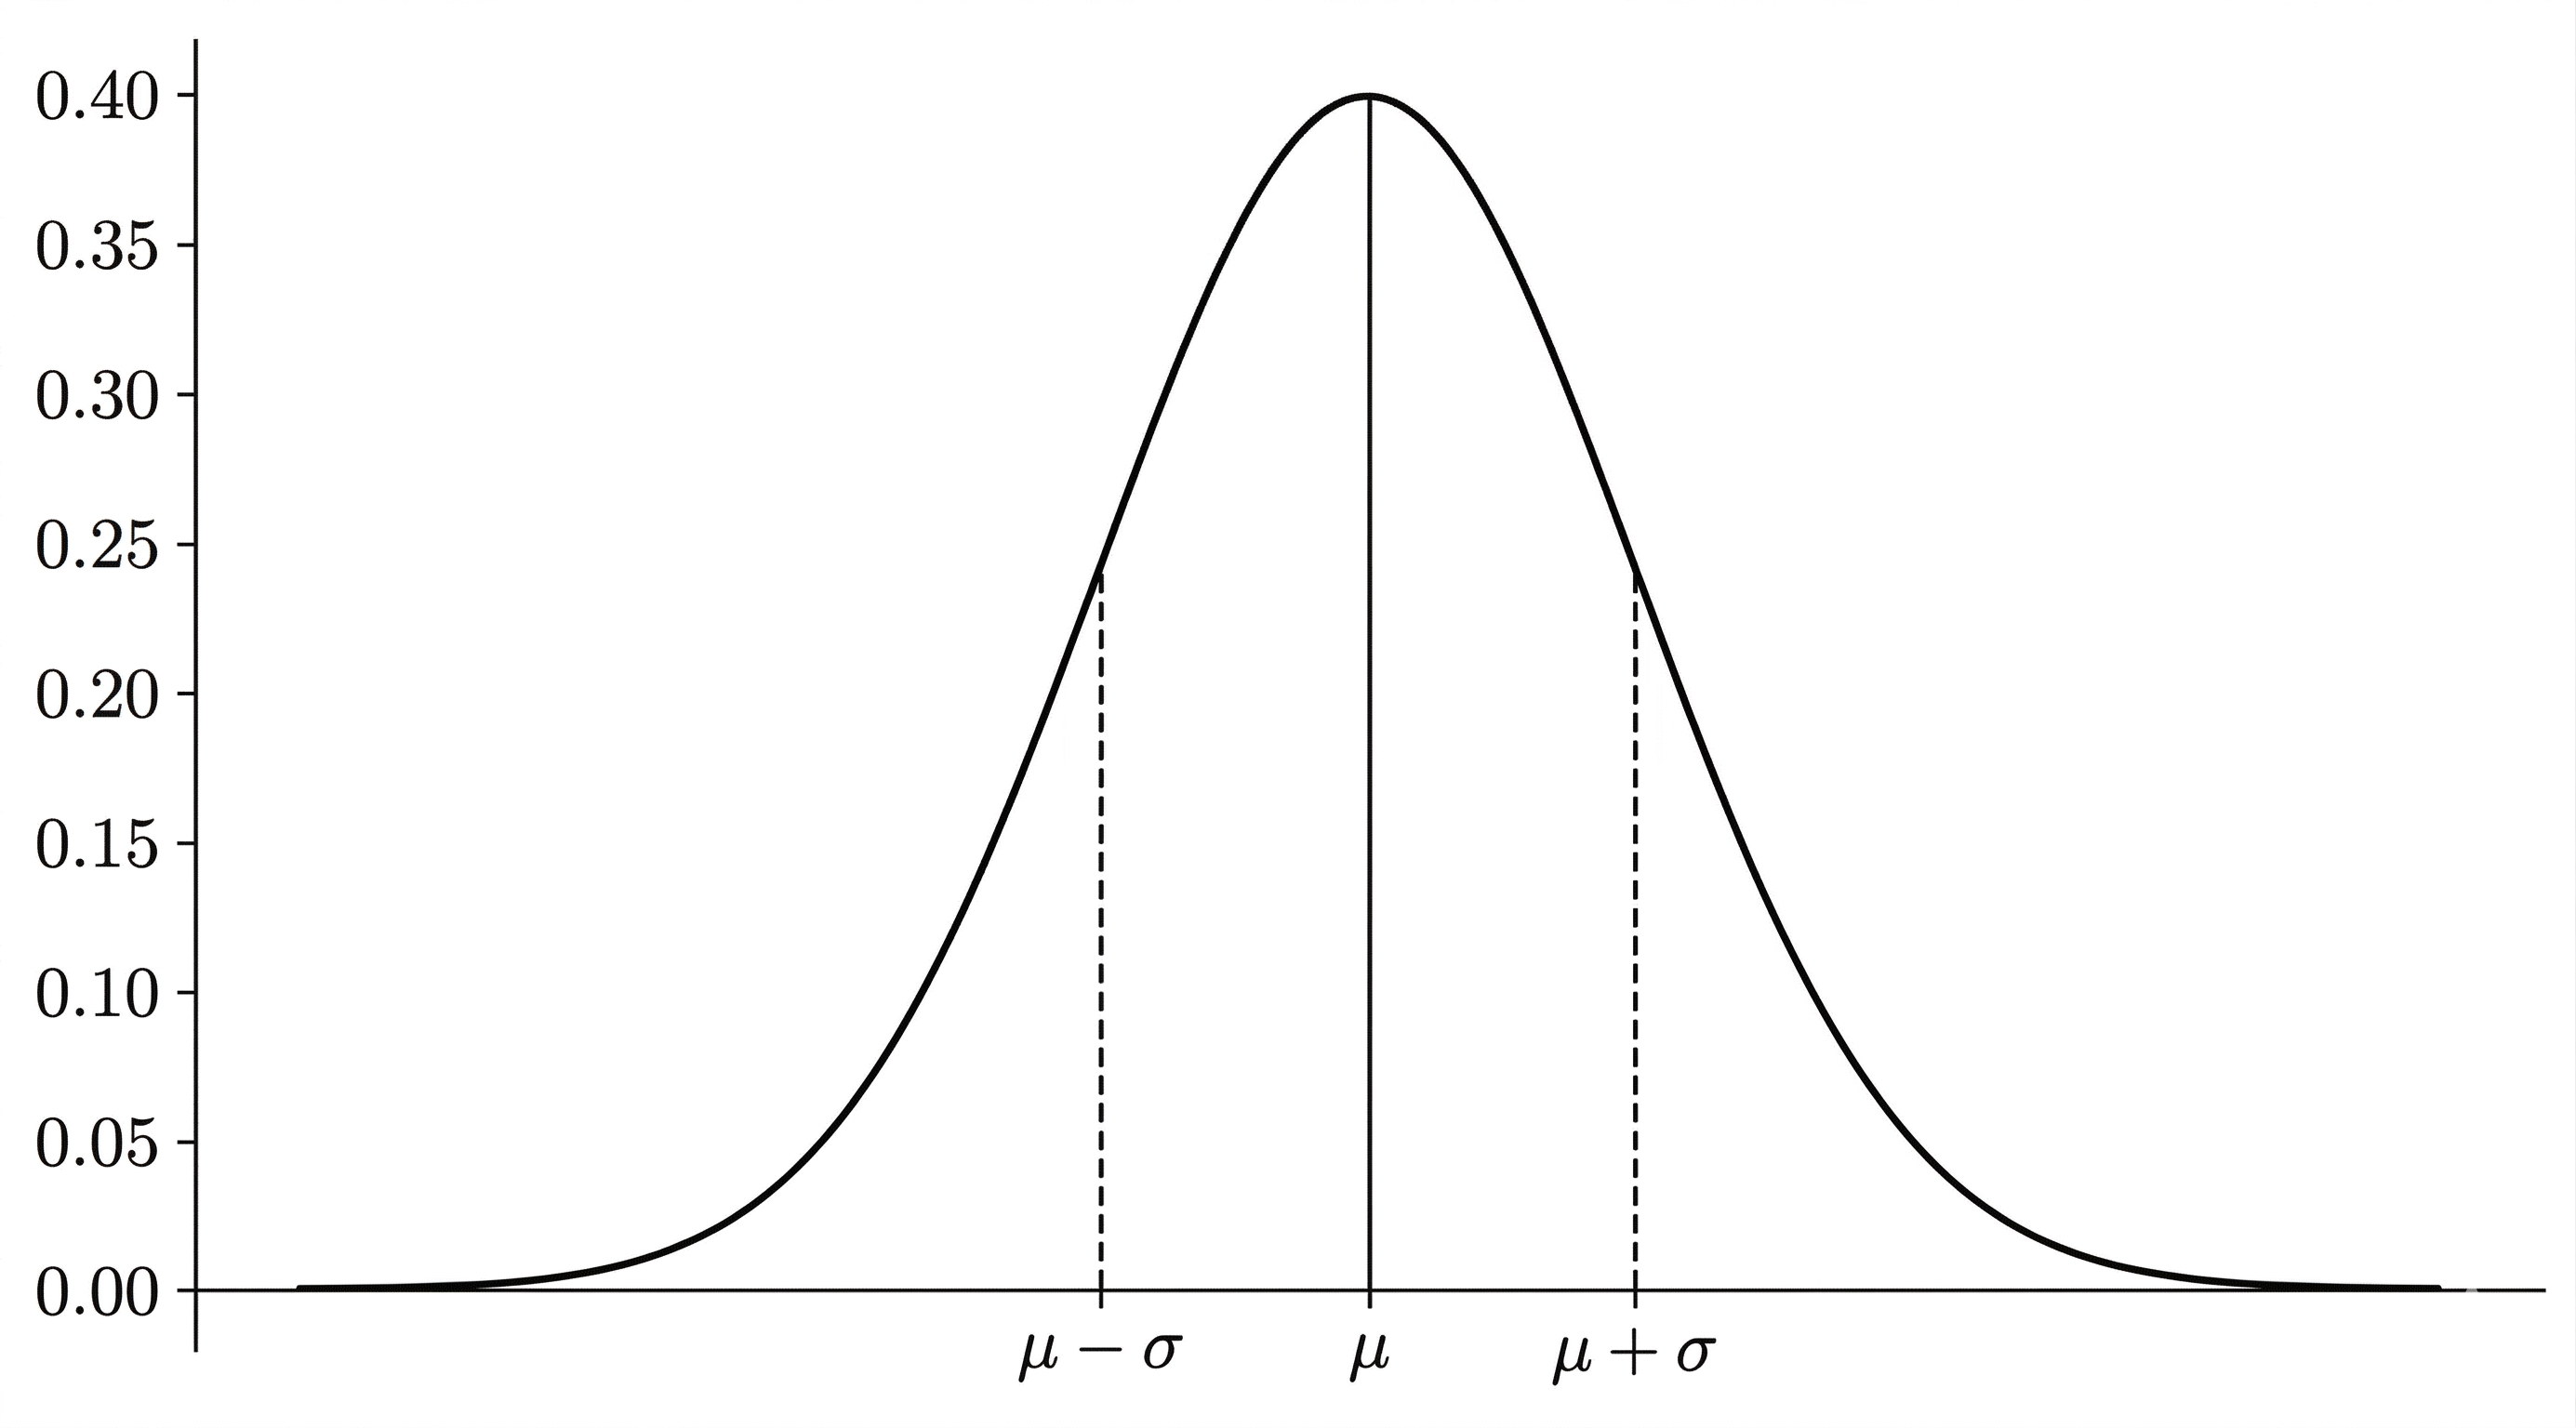
\includegraphics[width=0.6\textwidth]{figures/normal pdf.png}
    \caption{\label{fig:normal_pdf}Normal}
\end{figure}

Cuando tengamos una magnitud de entrada con distribución de origen normal no será necesario ``estandarizar'' la componente de incertidumbre con un factor de estandarización para obtener la incertidumbre típica, porque en ese caso la componente ya viene dada como la desviación estándar (o lo que es lo mismo, tenemos factor de estandarización 1).

La distribución uniforme o rectangular es una distribución de probabilidad continua que le asigna igual probabilidad a todos los resultados dentro de un intervalo $[a, b]$. Su función de densidad de probabilidad es:
\begin{equation}
    f(x) = \begin{cases}
        \frac{1}{b-a} & \text{si } a \leq x \leq b \\
        0 & \text{en otro caso}
    \end{cases}.
\end{equation}

El ancho de la curva es $\Delta = b-a$, la media es $\mu = \frac{a+b}{2}$ y la desviación estándar es $\sigma = \frac{b-a}{\sqrt{12}} = \frac{b-a}{2\sqrt{3}}$.

\begin{figure}[!htb]
    \centering
    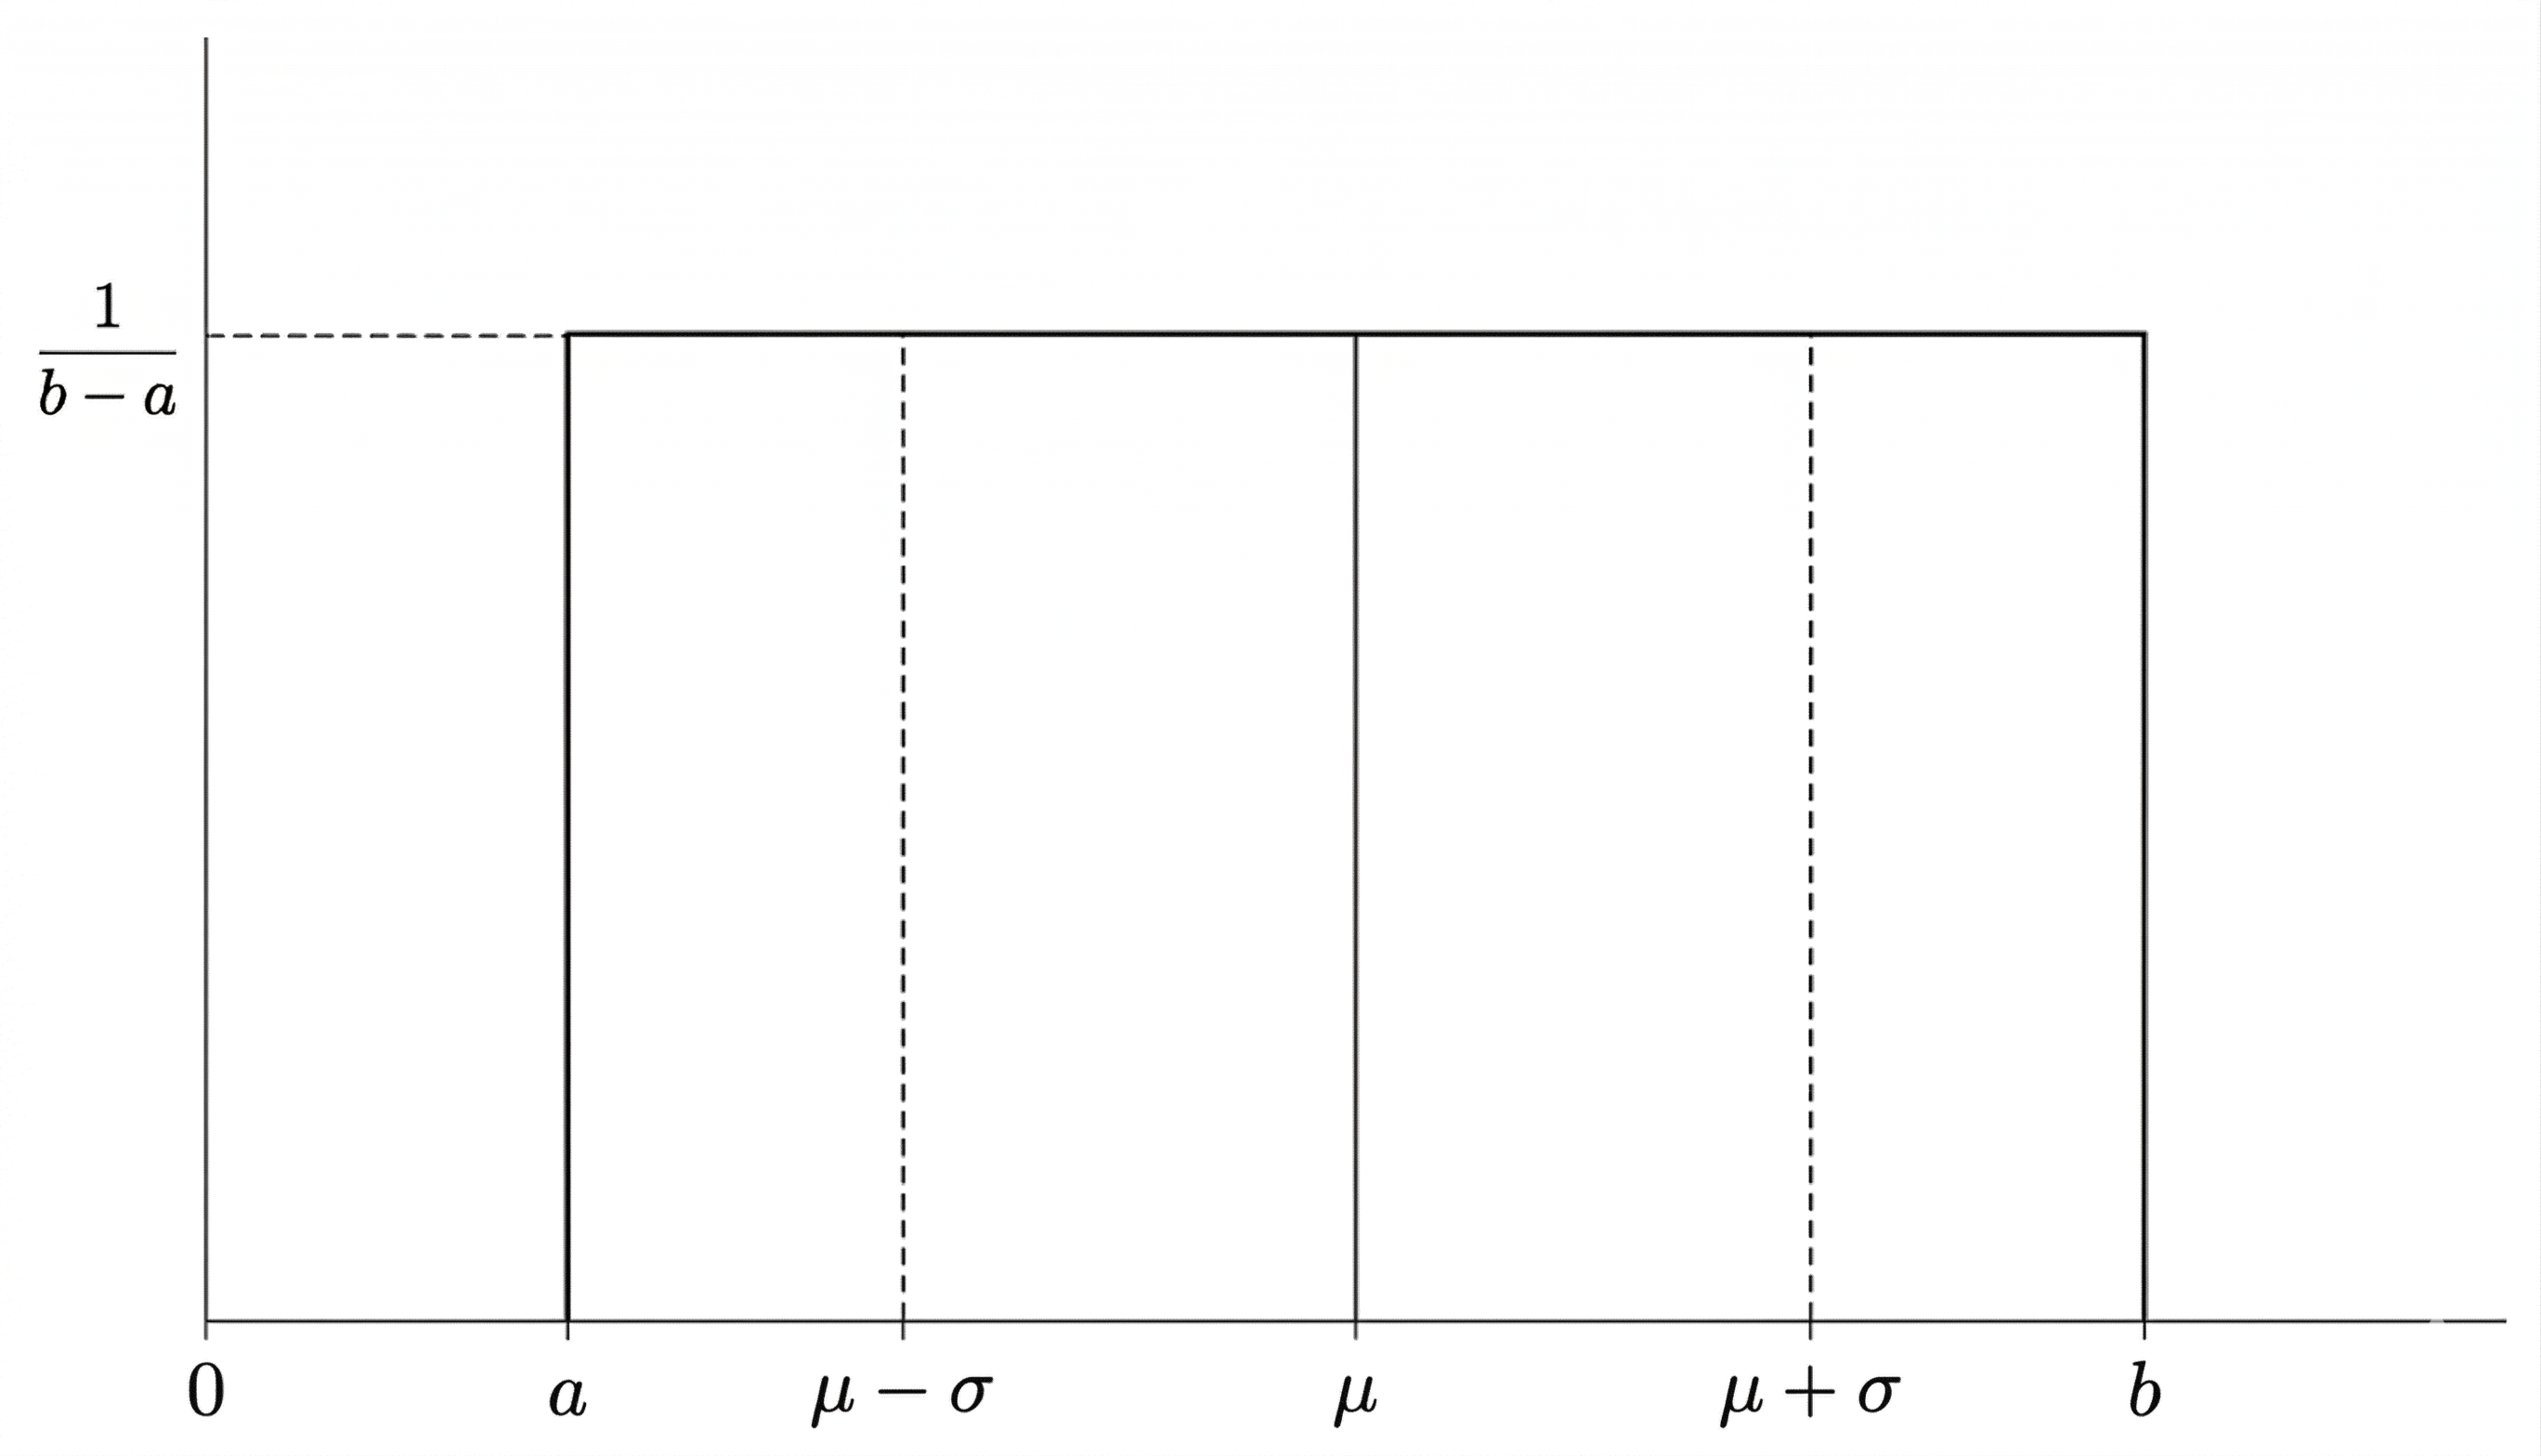
\includegraphics[width=0.6\textwidth]{figures/rectangular pdf.png}
    \caption{\label{fig:rectangular_pdf}Rectangular}
\end{figure}


Cuando tenemos una magnitud de entrada con distribución de origen rectangular, la componente de incertidumbre viene dada como el ancho $\Delta$ o el medio ancho $\frac{\Delta}{2}$ de la curva, y el factor de estandarización necesario para obtener la incertidumbre típica será $\frac{1}{\sqrt{12}}$ o $\frac{1}{\sqrt{3}}$ respectivamente.

La distribución triangular se usa cuando hay poca información disponible sobre la magnitud de entrada, y se conoce o interesa sólo el mínimo, el máximo y el valor más probable.

\begin{figure}[!htb]
    \centering
    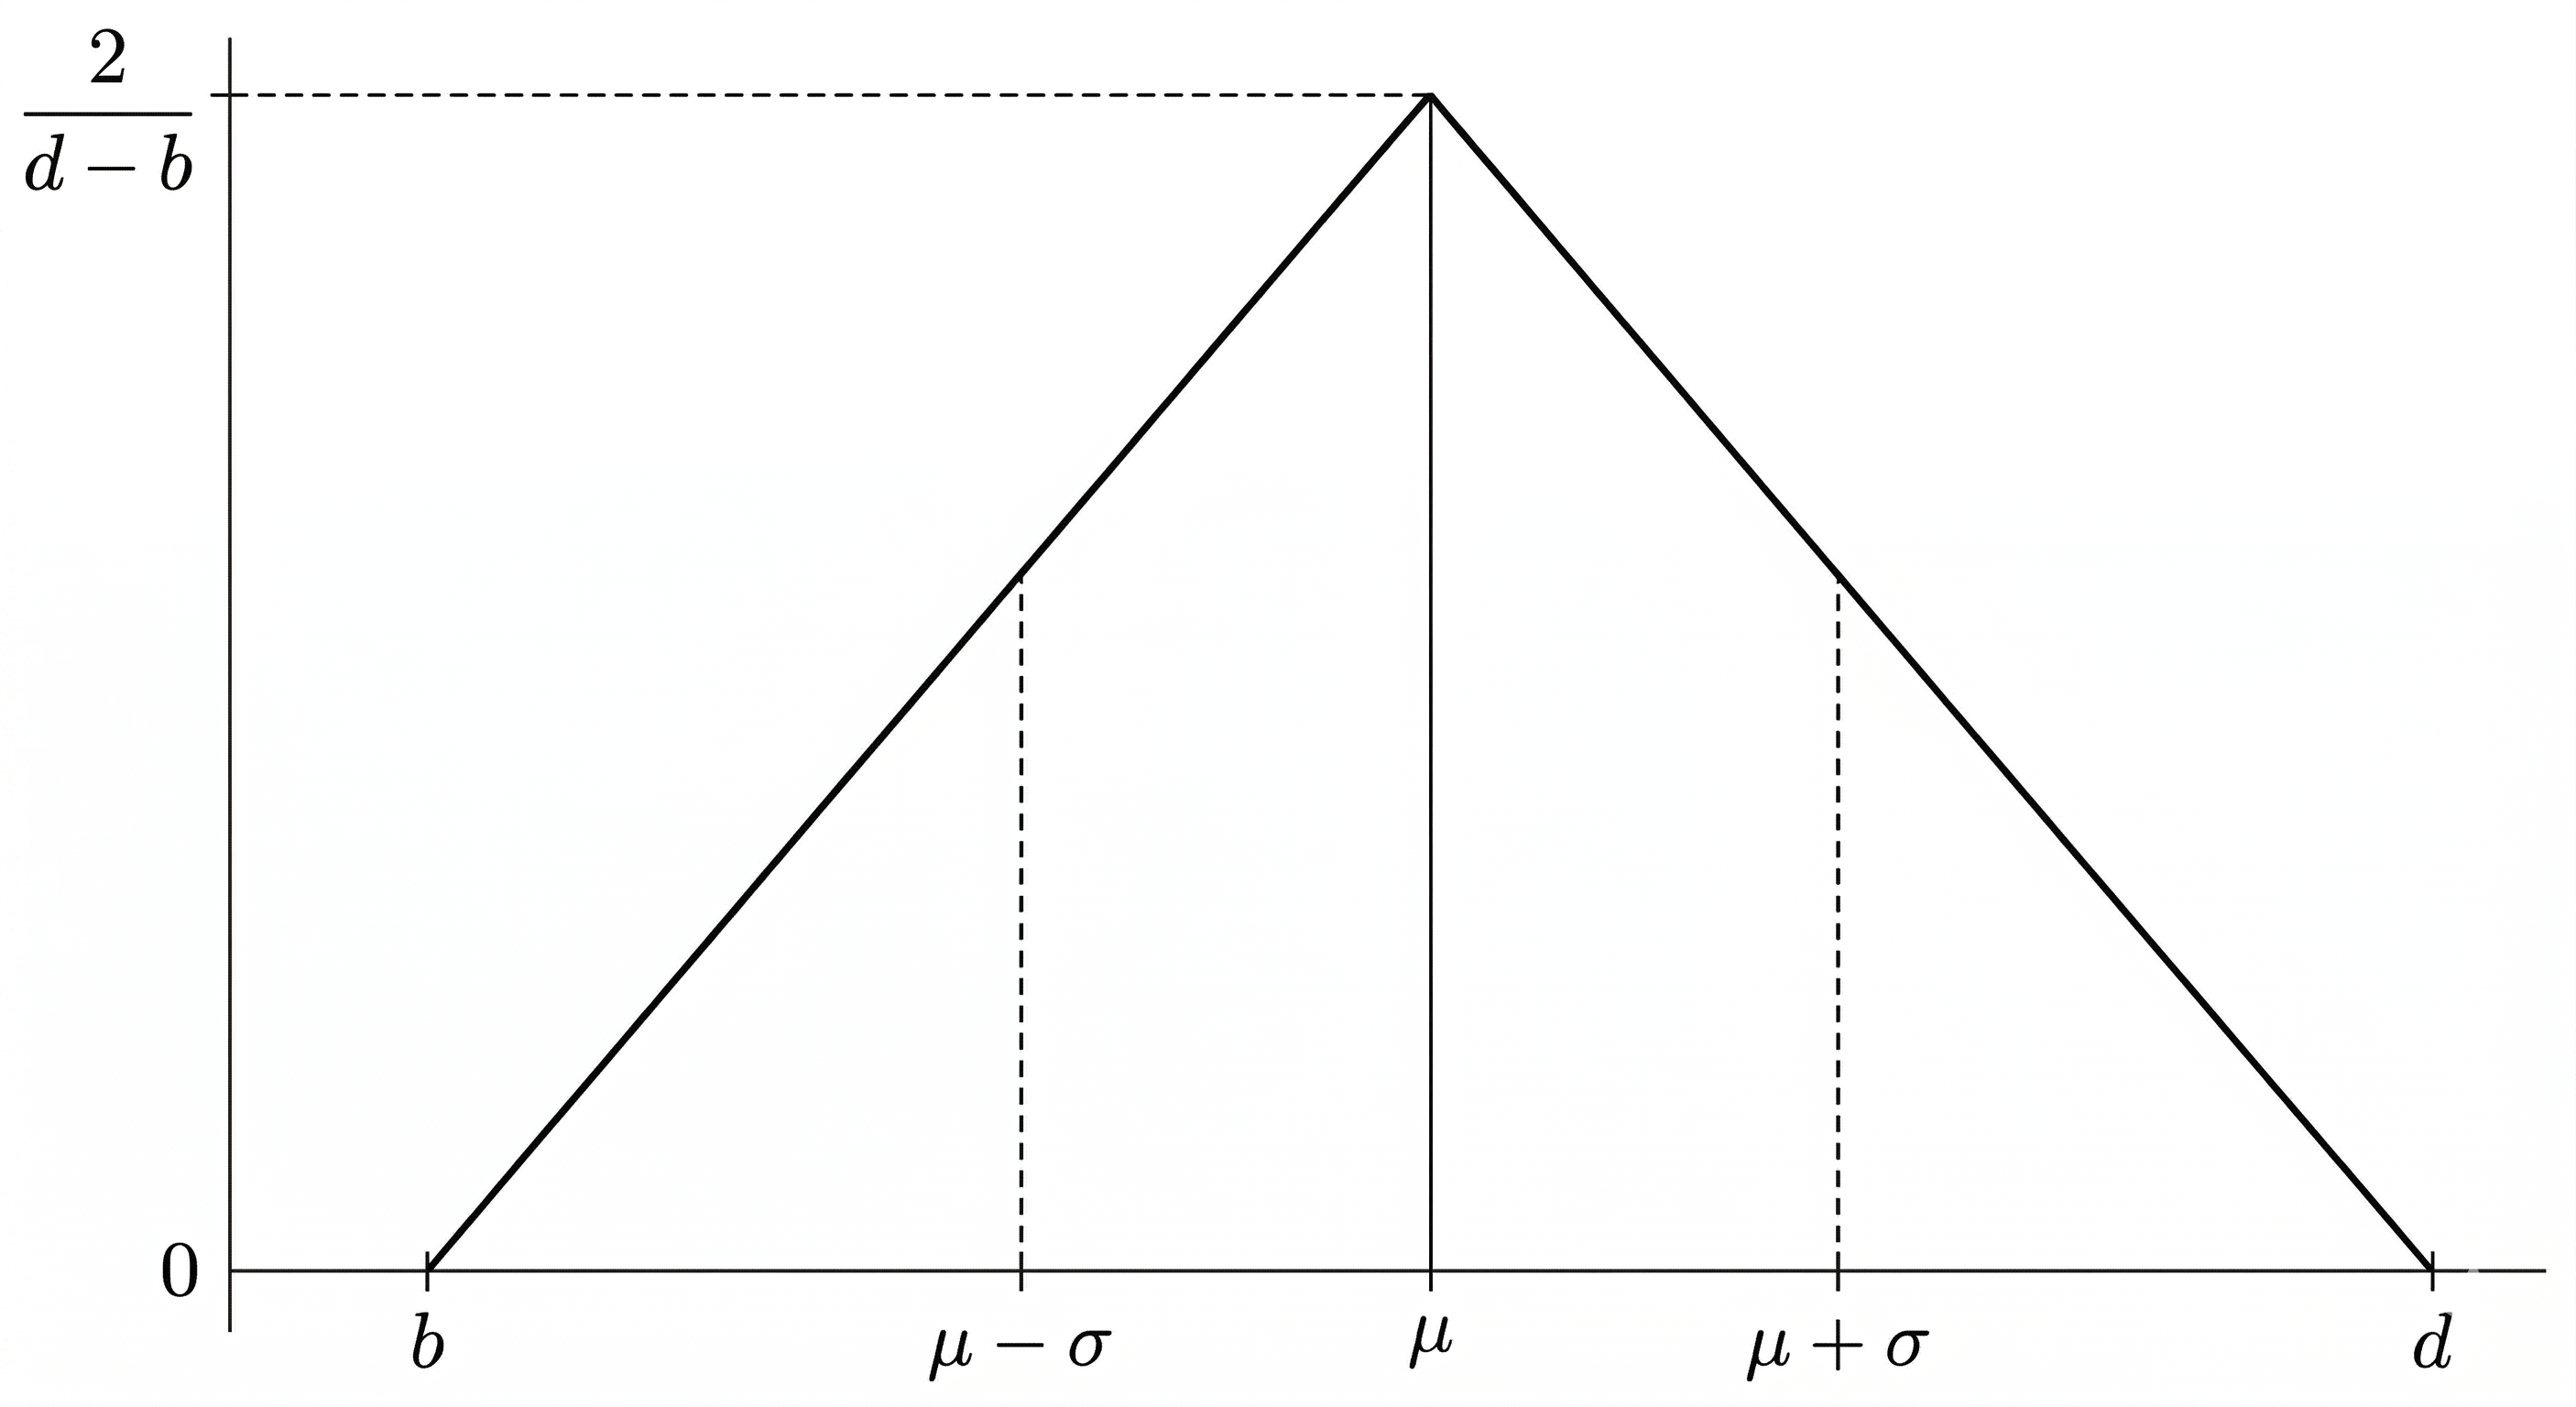
\includegraphics[width=0.6\textwidth]{figures/triangular pdf.png}
    \caption{\label{fig:triangular_pdf}Triangular}
\end{figure}

Cuando es simétrica respecto a la esperanza $\mu = \frac{b+d}{2}$, el ancho de la curva es $\Delta = d-b$ y la desviación estándar es $\sigma = \frac{d-b}{2\sqrt{6}}$. La componente de incertidumbre viene dada como el ancho $\Delta$ o el medio ancho $\frac{\Delta}{2}$ de la curva, y el factor de estandarización necesario para obtener la incertidumbre típica será $\frac{1}{2\sqrt{6}}$ o $\frac{1}{\sqrt{6}}$ respectivamente.

\section{Temperatura}\label{sec:temperatura}

\subsection{Determinación informada}

La determinación informada en el certificado (mensurando, resultado de salida) es la corrección de la UBP:
\begin{equation}
    C = T_{ref} - T_{med} = \left[\bar{T}_{pat} + \sum_i \delta_{\textit{ref, i}}\right]-\left[\bar{T}_{ubp} + \sum_j \delta_{\textit{ubp, j}}\right]
    \label{eq:correccion-temperatura}
\end{equation}

% **[INM §6.5.1, p.12 y ec. (1) p.13; th-001 §4, p.7-9 ec. (1)/(2) y §5.4.3, p.15 ec. (5).]**

donde $T_{ref}$ es la temperatura de referencia y $T_{med}$ la temperatura medida. La temperatura medida es el promedio de las mediciones de la UBP más las correcciones $\delta_{\textit{ubp, j}}$ que provienen de la UBP. La temperatura de referencia es el promedio de las mediciones del patrón más todas las correcciones restantes $\delta_{\textit{ref, i}}$: las que provienen del patrón y las que provienen del medio de comparación. Como consecuencia de la linealidad de la \cref{eq:correccion-temperatura} en las correcciones $\delta$,
\begin{equation}
    c_i = \frac{\partial C}{\partial \delta_i} = 1 \ \ y \ \ c_j = \frac{\partial C}{\partial \delta_j} = -1      
\end{equation}
es decir que el coeficiente de sensibilidad vale -1 para toda componente de incertidumbre que provenga de la UBP, y +1 para todas las demás: las del patrón y las del medio de comparación.

Las únicas correcciones que se consideran significativas son la corrección por polinomio interpolador del patrón y, en el caso de temperatura de contacto, la corrección por error de inmersión. El resto de las contribuciones se considera despreciable en corrección (tienen estimación nula), aunque aporten en la incertidumbre (ver sec.  Componentes de incertidumbre).

\textbf{Ambiental}

\begin{equation}
    C = \bar{T}_{pat} + \delta_{\textit{ccr pat}} - \bar{T}_{ubp}    
\end{equation}

\textbf{Contacto (alta y baja exactitud)}
\begin{equation}
    C = \bar{T}_{pat} + \delta_{\textit{ccr pat}} + \delta_{\textit{imm pat}} - (\bar{T}_{ubp} + \delta_{\textit{imm ubp}})
\end{equation}

\subsection{Correcciones}

\subsubsection{Corrección del patrón por polinomio de interpolación ($\delta_{\textit{ccr pat}}$)}

Los coeficientes $m$ y $b$ salen del ajuste lineal por mínimos cuadrados de la corrección informada en el certificado de calibración vigente del patrón. La corrección es la función de ajuste (recta) evaluada en el promedio de la temperatura medida por el patrón.
\begin{equation}
    \delta_{\textit{ccr pat}} = m\bar{T}_{pat} + b
\end{equation}

% **[GUM H.3.1-H.3.3, p.93-95; N&W §2.12, p.83-85]**

\subsubsection{Por error de inmersión ($\delta_{\textit{imm}}$)}
Aplica sólo para termómetros de contacto, que se calibran en medios de inmersión (bloques secos y baños líquidos). En termómetros con sensores de longitud no despreciable [nota acá: cuál es una long no despreciable?] se observa que la punta del termómetro está a una temperatura ligeramente diferente que el medio de interés, indicando temperaturas ligeramente inferiores en módulo. La corrección de este efecto se modela como

\begin{equation}
    \delta_{\textit{imm}} = (T_{set} - T_{amb})Ke^{\frac{-L}{D_{eff}}}
\end{equation}

donde $T_{set}$ es el punto de seteo, es decir la temperatura nominal del punto de calibración, $T_{amb}$ la temperatura ambiente, $K$ una constante aproximadamente igual a 1, $L$ la longitud de inmersión y $D_{eff}$ el diámetro efectivo del termómetro.
Para baños líquidos $D_{eff}$ = D, el diámetro del termómetro, y para bloques secos $D_{eff} = 2D$. Se puede reescribir como se muestra arriba definiendo una constante $\gamma$ = 1 ó 2 según si el medio es baño líquido o bloque seco. 
% **[N&W §4.4.1, p.137; Tavener §3, p.5, Tavener §3, p.6]**

La bibliografía sólo acota $K$ como una constante siempre menor que 1 pero próxima a la unidad, y traza las curvas del modelo tomando $K = 1$. En este modelo matemático se adopta ese mismo valor, $K = 1$, de modo que las correcciones que se aplican al patrón y a la UBP resultan
\begin{equation}
    \delta_{\textit{imm pat}} = (T_{set} - T_{amb})\,e^{\frac{-L_{pat}}{\gamma D_{pat}}} \ \ \ \ \delta_{\textit{imm ubp}} = (T_{set} - T_{amb})\,e^{\frac{-L_{ubp}}{\gamma D_{ubp}}}
\end{equation}

Para el caso de mediciones en laboratorio el patrón siempre se inserta a la inmersión máxima posible del medio ($L_{pat}$ = longitud de inmersión máxima del medio). Para la UBP se sobreestima la corrección asumiento que está a la inmersión mínima posible en el medio ($L_{ubp}$ = longitud de inmersión mínima del medio) ya que las longitudes de los sensores de la ubp pueden variar.

\subsection{Componentes de incertidumbre}

\textbf{Repetibilidad} ($\sigma_{\textit{rep ubp}}$, $\sigma_{\textit{rep pat}}$)

Incertidumbre asociada a tomar el promedio de una serie de mediciones como valor de la magnitud. Se calcula como la desviación estándar experimental de la media de las $n$ mediciones registradas en el punto de calibración, por separado para la UBP y para el patrón.
\begin{equation}
    \Delta_{\textit{rep ubp}} = s(\bar{T}) = \frac{s(T_k)}{\sqrt{n}} = \sqrt{\frac{\sum_{k=1}^{n}(T_k - \bar{T})^2}{n(n-1)}}
\end{equation}

% **[GUM 4.2.2, p.13 ec. (4); GUM 4.2.3, p.13 ec. (5); INM Tabla 2, p.14-15]**

\textbf{Resolución} ($\sigma_{\textit{res ubp}}$, $\sigma_{\textit{res pat}}$)

Incertidumbre debida a la mínima diferencia entre indicaciones que el instrumento puede distinguir. Para una indicación dada, el valor de la magnitud puede encontrarse con igual probabilidad en cualquier punto del intervalo de amplitud $R$ centrado en ella, de modo que la resolución $R$ declarada del instrumento es el ancho completo de una distribución rectangular y no requiere un cálculo adicional.

% **[GUM F.2.2.1, p.67; N&W §2.3.2, p.44 ec. (2.9)-(2.12)]**

\textbf{Histéresis} ($\sigma_{\textit{his ubp}}$)

Fenómeno que hace que la lectura del instrumento dependa de si el valor fue alcanzado en forma ascendente o descendente. Sin información sobre la exposición previa del termómetro, la mejor representación es una distribución rectangular cuyo ancho completo es la amplitud del lazo de histéresis. Se aplica uno de dos criterios.

\textit{Criterio 1} (por defecto): Se asume el 0,2\% del rango ensayado, extremo pesimista del rango de histéresis típico de las termorresistencias industriales:

\begin{equation}
    \Delta_{\textit{his ubp}} = 0{,}002\,(T_{max} - T_{min}),
\end{equation}

donde $T_{max}$ y $T_{min}$ son el mayor y el menor punto de calibración ensayados. Al obtenerse de información previa y no de una serie de mediciones, es de tipo B.

% **[th-001 §4, p.6; DKD-R 5-1 §8.10, p.19; N&W §2.7.3 Ej. 2.10, p.61]**

\textit{Criterio 2}: Se registran mediciones en el punto medio del rango durante la carrera ascendente y nuevamente al descender desde el valor máximo, y la histéresis es la diferencia entre los promedios de ambas series:

\begin{equation}
    \Delta_{\textit{his ubp}} = \lvert \bar{T}_{asc} - \bar{T}_{desc} \rvert.
\end{equation}

Al obtenerse del análisis estadístico de series de observaciones es de tipo A, con $\nu = 2n-2$: dos series de $n$ mediciones y dos restricciones, una por cada promedio.

% **[N&W §2.7.3 Ej. 2.10, p.62-63; DKD-R 5-1 §8.10, p.18-19; INM Tabla 4, p.20]**

\textbf{Incertidumbre por interpolación de la corrección del patrón} ($\sigma_{\textit{int ccr pat}}$)

Incertidumbre de haber obtenido la corrección del patrón (sec. 2.2.1) mediante un ajuste por mínimos cuadrados. No es la incertidumbre de la corrección interpolada, sino la del método de ajuste empleado, y se mide por la dispersión de los residuos:

\begin{equation}
    \Delta_{\textit{int ccr pat}} = \sqrt{\frac{\sum_{k=1}^{n}\left[ C_k - C(T_k) \right]^2}{n-2}},
\end{equation}

donde $C_k$ son las correcciones informadas en el certificado de calibración del patrón, $C(T_k)$ las predichas por la recta de ajuste evaluada en las mismas temperaturas, y $n$ el número de puntos del certificado. Se resta 2 por los dos parámetros del ajuste lineal.

% **[GUM H.3.2, p.94 ec. (H.13f) y p.95; GUM G.3.3, p.76-77; N&W §2.12.1, p.85 ec. (2.73); INM §6.5.2, p.28 ec. (13); th-001 §6.1.1, p.17]**

\textbf{Incertidumbre de calibración del patrón} ($\sigma_{\textit{cal pat}}$)

Incertidumbre de medición del patrón informada en su certificado de calibración, evaluada en la temperatura de referencia del punto. Como el certificado informa la incertidumbre en un número acotado de puntos, se ajusta un polinomio cuadrático a esos valores y se lo evalúa en $T_{ref}$. El resultado es una incertidumbre expandida, de modo que se divide por el factor de cobertura $k=2$ con el que fue informada para obtener la incertidumbre estándar:

\begin{equation}
    \Delta_{\textit{cal pat}} = \frac{a\,T_{ref}^2 + b\,T_{ref} + c}{2},
\end{equation}

donde $a$, $b$ y $c$ son los coeficientes del ajuste cuadrático de la incertidumbre expandida del certificado en función de la temperatura.

% **[GUM 4.3.3, p.15; GUM F.2.3.1, p.68; N&W §2.11-2.12, p.77-85; th-001 §6.1.1, p.16; th-003 §6.1 2), p.23; INM Tabla 2, p.14]**

\textbf{Incertidumbre por interpolación de la incertidumbre de calibración del patrón} ($\sigma_{\textit{int cal pat}}$)

Análoga a la interpolación de la corrección, pero sobre el ajuste cuadrático de la componente anterior: es la incertidumbre de haber empleado el método de mínimos cuadrados para conocer la incertidumbre de calibración en puntos intermedios.

\begin{equation}
    \Delta_{\textit{int cal pat}} = \frac{1}{2}\sqrt{\frac{\sum_{k=1}^{n}\left[ U_k - U(T_k) \right]^2}{n-3}},
\end{equation}

donde $U_k$ son las incertidumbres expandidas informadas en el certificado y $U(T_k)$ las predichas por el ajuste. Se resta 3 por los tres parámetros del ajuste cuadrático, y se divide por 2 porque los datos ajustados son incertidumbres expandidas con $k=2$.

% **[GUM H.3.2, p.94 ec. (H.13f); GUM G.3.3, p.76-77; N&W §2.12.1, p.85 ec. (2.73); INM §6.5.2, p.28 ec. (13)]**

\textbf{Deriva del patrón} ($\sigma_{\textit{der pat}}$)

Incertidumbre asociada a la variación de la lectura del patrón con el tiempo, entre calibraciones sucesivas. Se estima como un tercio de la \textit{tolerancia del patrón} —su especificación de fábrica— evaluada en la temperatura de referencia, declarada como medio ancho de una distribución rectangular:

\begin{equation}
    \Delta_{\textit{der pat}} = \frac{tol_{\textit{pat}}}{3} = \frac{1}{3}\left( \frac{tol_{p,\textit{pat}}\%}{100}\lvert T_{ref} \rvert + tol_{f,\textit{pat}} \right),
\end{equation}

donde $tol_{p,\textit{pat}}$ y $tol_{f,\textit{pat}}$ son la tolerancia porcentual y la tolerancia fija especificadas por el fabricante del patrón. No debe confundirse con la tolerancia de calibración de la sec. 1.5.3, que la solicita el cliente para cada punto y se evalúa en el punto de seteo $T_{set}$.

%**[th-001 §6.1.1, p.16-17; th-003 §6.1 2), p.23; INM §6.5.2, p.28]**

\textbf{Inestabilidad del medio} ($\sigma_{\textit{ine med}}$)

Incertidumbre debida a la variación de la temperatura del medio de comparación en el tiempo durante la medición. Se obtiene evaluando la temperatura de referencia en la recta de ajuste de la inestabilidad medida en la caracterización del medio, con los coeficientes correspondientes al rango que contiene al punto de calibración:

\begin{equation}
    \Delta_{\textit{ine med}} = m_{ine}\,T_{ref} + b_{ine}.
\end{equation}

% **[INM §6.5.1.1, p.13 y Tabla 2, p.14; th-003 §6.1 2), p.23]**

\textbf{Inhomogeneidad axial del medio} ($\sigma_{\textit{ina med}}$)

Incertidumbre debida a la variación de la temperatura a lo largo de la profundidad de los orificios del inserto de un bloque seco. Se obtiene igual que la inestabilidad, evaluando la temperatura de referencia en la recta de ajuste correspondiente de la caracterización del medio:

\begin{equation}
    \Delta_{\textit{ina med}} = m_{ina}\,T_{ref} + b_{ina}.
\end{equation}


% **[INM §6.5.1.2, p.16-17 y Tabla 3, p.17]**

\textbf{Inhomogeneidad radial del medio} ($\sigma_{\textit{inr med}}$)

Incertidumbre debida a la variación de la temperatura entre los distintos orificios del inserto de un bloque seco:

\begin{equation}
    \Delta_{\textit{inr med}} = m_{inr}\,T_{ref} + b_{inr}.
\end{equation}

% **[INM §6.5.1.2, p.16-17 y Tabla 3, p.17]**

\textbf{Inhomogeneidad volumétrica del medio} ($\sigma_{\textit{inv med}}$)

Incertidumbre debida a la variación de la temperatura dentro del volumen o zona de trabajo caracterizada de un baño líquido o de una cámara de temperatura ambiental:

\begin{equation}
    \Delta_{\textit{inv med}} = m_{inv}\,T_{ref} + b_{inv}.
\end{equation}
% **[INM §6.5.1.1, p.14 y Tabla 2, p.14; th-003 §6.1 2), p.24]**
\begin{table}[!htb]
\centering
\caption{Tabla de componentes de incertidumbre para calibraciones de temperatura de contacto y ambiental. En violeta se pintan las componentes correspondientes a la UBP, en amarillo las relacionadas al patrón y en rojo las que provienen del medio.}
\label{tab:my-table}
\resizebox{\textwidth}{!}{%
\begin{tabular}{|Qc|Qc|Qc|Qc|Qc|Qc|Qc|Qc|}
\hline
 &
  \textbf{Componente} &
  \textbf{Valor $(\Delta)$} &
  \textbf{Distribución} &
  \textbf{Factor} &
  \textbf{Tipo} &
  \textbf{\begin{tabular}[c]{@{}c@{}}Grados de \\ libertad\end{tabular}} &
  \textbf{$c_i$} \\ \hline
\rowcolor[HTML]{ECF4FF} 
1 &
  $\sigma_{\textit{rep ubp}}$ &
  $\dfrac{s_{ubp}}{\sqrt{n}}$ &
  Normal &
  1 &
  A &
  $n-1$ &
  -1 \\ \hline
\rowcolor[HTML]{ECF4FF} 
2 &
  $\sigma_{\textit{res ubp}}$ &
  $\sigma_{\textit{res ubp}}$ &
  \begin{tabular}[c]{@{}c@{}}Rectangular, \\ ancho completo\end{tabular} &
  $2\sqrt{3}$ &
  B &
  100 &
  -1 \\ \hline
\rowcolor[HTML]{ECF4FF} 
\cellcolor[HTML]{ECF4FF} &
  \cellcolor[HTML]{ECF4FF} &
  Crit. 1: $0.2\%\cdot (T_{max}-T_{min})$ &
  \cellcolor[HTML]{ECF4FF} &
  \cellcolor[HTML]{ECF4FF} &
  B &
  100 &
  \cellcolor[HTML]{ECF4FF} \\ \cline{3-3} \cline{6-7}
\rowcolor[HTML]{ECF4FF} 
\multirow{-2}{*}{\cellcolor[HTML]{ECF4FF}3} &
  \multirow{-2}{*}{\cellcolor[HTML]{ECF4FF}$\sigma_{\textit{his ubp}}$} &
  Crit. 2: $\lvert \bar{T}_{asc}-\bar{T}_{desc} \rvert$ &
  \multirow{-2}{*}{\cellcolor[HTML]{ECF4FF}\begin{tabular}[c]{@{}c@{}}Rectangular,\\ ancho completo\end{tabular}} &
  \multirow{-2}{*}{\cellcolor[HTML]{ECF4FF}$2\sqrt{3}$} &
  A &
  $2n-2$ &
  \multirow{-2}{*}{\cellcolor[HTML]{ECF4FF}-1} \\ \hline
\rowcolor[HTML]{FFFFC7} 
4 &
  $\sigma_{\textit{rep pat}}$ &
  $\dfrac{s_{pat}}{\sqrt{n}}$ &
  Normal &
  1 &
  A &
  $n-1$ &
  1 \\ \hline
\rowcolor[HTML]{FFFFC7} 
5 &
  $\sigma_{\textit{res pat}}$ &
  $\Delta_{\textit{res pat}}$ &
  \begin{tabular}[c]{@{}c@{}}Rectangular,\\ ancho completo\end{tabular} &
  $2\sqrt{3}$ &
  B &
  100 &
  1 \\ \hline
\rowcolor[HTML]{FFFFC7} 
6 &
  $\sigma_{\textit{int ccr pat}}$ &
  $\sqrt{\dfrac{\sum \textit{Residuos}^2}{n-2}}$ &
  Normal &
  1 &
  A &
  $n-2$ &
  1 \\ \hline
\rowcolor[HTML]{FFFFC7} 
7 &
  $\sigma_{\textit{cal pat}}$ &
  $\dfrac{a\cdot T_{ref}^2 + b\cdot T_{ref} + c}{2}$ &
  Normal &
  1 &
  B &
  100 &
  1 \\ \hline
\rowcolor[HTML]{FFFFC7} 
8 &
  $\sigma_{\textit{int cal pat}}$ &
  $\dfrac{1}{2}\sqrt{\dfrac{\sum \textit{Residuos}^2}{n-3}}$ &
  Normal &
  1 &
  A &
  $n-3$ &
  1 \\ \hline
\rowcolor[HTML]{FFFFC7} 
9 &
  $\sigma_{\textit{der pat}}$ &
  $\dfrac{1}{3}\left(\dfrac{tol_{\textit{\% pat}}}{100}\cdot \lvert T_{ref}\rvert + tol_{\textit{set pat}}\right)$ &
  \begin{tabular}[c]{@{}c@{}}Rectangular,\\ medio ancho\end{tabular} &
  $\sqrt{3}$ &
  B &
  100 &
  1 \\ \hline
\rowcolor[HTML]{FFCCC9} 
10 &
  $\sigma_{\textit{ine med}}$ &
  $m_{ine}\cdot T_{ref} + b_{ine}$ &
  \begin{tabular}[c]{@{}c@{}}Rectangular,\\ medio ancho\end{tabular} &
  $\sqrt{3}$ &
  B &
  100 &
  1 \\ \hline
\rowcolor[HTML]{FFCCC9} 
11 &
  $\sigma_{\textit{ina med}}$ &
  $m_{ina}\cdot T_{ref} + b_{ina}$ &
  \begin{tabular}[c]{@{}c@{}}Rectangular,\\ medio ancho\end{tabular} &
  $\sqrt{3}$ &
  B &
  100 &
  1 \\ \hline
\rowcolor[HTML]{FFCCC9} 
12 &
  $\sigma_{\textit{inr med}}$ &
  $m_{inr}\cdot T_{ref} + b_{inr}$ &
  \begin{tabular}[c]{@{}c@{}}Rectangular,\\ medio ancho\end{tabular} &
  $\sqrt{3}$ &
  B &
  100 &
  1 \\ \hline
\rowcolor[HTML]{FFCCC9} 
13 &
  $\sigma_{\textit{inv med}}$ &
  $m_{inv}\cdot T_{ref} + b_{inv}$ &
  \begin{tabular}[c]{@{}c@{}}Rectangular,\\ medio ancho\end{tabular} &
  $\sqrt{3}$ &
  B &
  100 &
  1 \\ \hline
\end{tabular}%
}
\end{table}

% \bibliographystyle{alpha}
% \bibliography{sample}
\printbibliography
\end{document}